\documentclass[11pt]{article}

\usepackage[margin=1in]{geometry}
\usepackage{amsmath,amssymb,mathtools}
\usepackage{booktabs}
\usepackage{enumitem}
\usepackage{hyperref}
\usepackage{microtype}
\usepackage{xcolor}
\usepackage{graphicx}

\newcommand{\ket}[1]{\lvert #1\rangle}

\hypersetup{
  colorlinks=true,
  linkcolor=blue!55!black,
  citecolor=blue!55!black,
  urlcolor=blue!55!black
}

\title{Methodology: QFT-Layout Quantum Neural Network Function Learning}
\author{QFT-Initialized Quantum Neural Network Research Lab}
\date{Protocol version 0.1 --- \today}

\begin{document}
\maketitle

\begin{abstract}
This protocol studies whether a two-qubit variational circuit initialized with randomized parameters can recover a known quantum Fourier transform (QFT), and whether it can perform a target function task even when it does not recover that full unitary. These are distinct outcomes. Circuit recovery is evaluated against the canonical QFT on the full operation; task performance is evaluated on held-out input--target examples and, where relevant, on recovered frequencies. Neither outcome is inferred from the other. The central aim is to understand these outcomes for declared circuit and encoding choices, not to search for a universally best ansatz.
\end{abstract}

\section{Research question and scope}

The primary question has two branches: (a) do randomized parameters converge to the canonical two-qubit QFT, and (b) if not, can the circuit still perform a specified function task with accurate held-out predictions and frequency recovery? A low task MSE is not evidence of QFT recovery; high QFT fidelity is not by itself evidence of learning an unknown function from examples. The function experiments so far are bounded proofs of concept and do not establish arbitrary-function learning or quantum advantage.

Keep direct circuit recovery and supervised task learning as separately labeled protocols. A QFT-recovery run may train against the canonical unitary or its action on a complete input basis, and must report full-unitary process fidelity. A function-learning run trains only on pairs $(x,y)$ with MSE and uses QFT fidelity only as a post-training diagnostic. For the latter, canonical QFT parameters and the target function's analytic spectrum are retained for analysis, but are never supplied to the optimizer. Report both branches when comparing whether task success occurs without convergence to QFT.

The research objective is not to select whichever circuit performs best. Preserve the baseline QFT-layout trainable block and state every encoding/depth change as an experimental factor. The lab will decide which factor to study next after reviewing the current evidence. In particular, a fixed alternative encoding can be compared while holding the trainable gate layout and parameter count constant. This keeps the trainable ansatz fixed in the narrow sense, although the encoding still changes the overall model's function class. Re-uploading the input between trainable blocks is a separate architecture change; if block count also changes, parameter count and depth are confounds that require a matched control.

\section{Model}

\subsection{Input domain and encoding}

The initial task is one-dimensional periodic regression on the unit circle, represented by $x\in[0,1)$, with period one. The baseline encoding is fixed, not learned: encode the scalar on qubit 0 as
\begin{equation}
  E(x) = R_y(2\pi x)\ket{0}
       = \cos(\pi x)\ket{0}+\sin(\pi x)\ket{1}.
  \label{eq:encoding}
\end{equation}
Qubit 1 starts in $\ket{0}$, so the two-qubit input is
\begin{equation}
  \ket{\psi(x)} = E(x)\otimes\ket{0}.
\end{equation}
This is a unitary angle encoding with inverse $R_y(-2\pi x)$. The domain is periodic: $x=0$ and $x=1$ denote the same point and must not be treated as distinct examples. Retain the original classical $x$ in the dataset and run bundle. The encoding operation is reversible on the stated domain; this does not imply that measuring the encoded state can recover an arbitrary continuous $x$ exactly.

\subsection{Trainable QFT-layout block and readout}

Apply the seven-parameter circuit
\begin{equation}
  V(\boldsymbol{\theta}) = \operatorname{SWAP}_{0,1}
  \bigl(U_0(\theta_4,\theta_5,\theta_6)\bigr)
  \operatorname{CP}_{1\rightarrow0}(\theta_3)
  \bigl(U_1(\theta_0,\theta_1,\theta_2)\bigr),
  \label{eq:ansatz}
\end{equation}
where $U_j(\theta,\phi,\lambda)$ is the standard single-qubit Euler gate and $\operatorname{CP}$ is the controlled-phase gate. The circuit order is the QFT-layout order: $U$ on wire 1, controlled phase from wire 1 to wire 0, $U$ on wire 0, then the final bit-reversal SWAP. The ansatz has the same gate layout as the reference two-qubit QFT, with trainable gate angles. It is not constrained to remain the exact QFT during function training.

The model returns the ideal expectation of Pauli $Z$ on wire 1 after the variational block:
\begin{equation}
  f_{\boldsymbol{\theta}}(x)
  = \bra{\psi(x)}V(\boldsymbol{\theta})^\dagger
    (I_0\otimes Z_1)V(\boldsymbol{\theta})\ket{\psi(x)}.
  \label{eq:readout}
\end{equation}
Thus $f_{\boldsymbol{\theta}}(x)\in[-1,1]$. This first protocol uses exact statevector expectation values, without shot noise or hardware noise. Finite-shot and noisy variants are separate, explicitly labeled experiments.

Encoding is a declared model factor. A sweep over predetermined encodings (for example, integer-scaled $R_y(2\pi kx)$ maps for a period-one domain) can hold this seven-parameter trainable block fixed. Do not describe such a sweep as learning the encoding. An integer scale preserves period one, but a single scaled rotation does not generally provide an arbitrary mixture of harmonics. Re-uploading $x$ between trainable blocks is a different factor because it changes the input-dependent circuit structure; if repeated blocks add trainable parameters, compare against a matched-depth single-upload control before attributing gains to re-uploading. Repeated data encoding and its relationship to accessible Fourier frequencies are established topics in variational quantum learning \cite{schuld2021,perez2020}.

\section{Fabricated data}

Use a versioned deterministic generator to create a period-one target from a finite real Fourier expansion:
\begin{equation}
  g(x)=a_0+\sum_{k\in\mathcal{K}}
  \left[a_k\cos(2\pi kx)+b_k\sin(2\pi kx)\right].
  \label{eq:target}
\end{equation}
For the first run, use a single nonzero frequency $k=1$ (plus an optional constant offset), with coefficients chosen so that $g(x)\in[-1,1]$. This is the conservative initial target for a single angle upload. A later complexity ladder should introduce additional frequencies and higher bandwidth only as separately configured experiments. The accessible spectrum depends on the encoding and the number and placement of data uploads; a shallow model with one upload should not be assumed to represent arbitrary spectra \cite{schuld2021}.

Generate fixed train, validation, and test inputs with independent, recorded seeds. Sample the base splits uniformly on $[0,1)$; avoid duplicating periodic endpoints. Evaluate analytic target values from Equation~\eqref{eq:target}. Keep the split membership fixed across optimizer and initialization comparisons. Training uses only the training split. Validation data may guide a predeclared stopping rule or model selection. Test data are evaluated only for final reporting. The target coefficients and exact spectrum are evaluation metadata, not training features.

Store the generator name and version, target family and coefficients, domain, all seeds, sample counts, split IDs, and the actual input and target arrays. For small experiments, save arrays in a non-pickle NumPy \texttt{.npz} file, with a JSON manifest describing keys, shapes, dtypes, units, and split semantics.

\section{Training objective and procedure}

Given training examples $\mathcal{D}_{\mathrm{train}}=\{(x_i,y_i)\}_{i=1}^{N}$ with $y_i=g(x_i)$, train the circuit parameters by minimizing empirical MSE:
\begin{equation}
  \mathcal{L}_{\mathrm{train}}(\boldsymbol{\theta})
  = \frac{1}{N}\sum_{i=1}^N
    \left(f_{\boldsymbol{\theta}}(x_i)-y_i\right)^2.
  \label{eq:mse}
\end{equation}
Do not add a process-fidelity term, parameter-distance-to-QFT term, or frequency-label term to this first objective. Those would provide additional information beyond ordinary supervised regression. The optimizer sees only input--target pairs and the MSE. Use a seeded random initialization of the seven circuit parameters, with the initialization distribution and range recorded in the resolved configuration. Do not initialize around the canonical QFT angles for this function-learning protocol.

The training implementation must record loss histories and parameter values by optimization step. Use a fixed optimizer, learning rate, stopping rule, and evaluation budget in the initial baseline; subsequent optimizer studies must hold data, split IDs, seeds, initialization distribution, and budgets fixed. Report optimizer steps and objective/circuit evaluations, since a step is not a uniform measure of compute across optimizers. If analytic gradients are used in the ideal simulator, record that fact and the gradient method.

\section{Evaluation and baselines}

At the final declared checkpoint, calculate train, validation, and test MSE separately. Also report test RMSE and $R^2$ (with the constant-target edge case handled explicitly). The test score is the task-performance endpoint. Report results for every seed, including failures and incomplete runs, rather than selecting the best seed.

Measure spectral recovery independently of training loss. Evaluate the model and target on a fixed dense uniform grid over $[0,1)$; estimate their Fourier coefficients using the same declared discrete Fourier convention, and report coefficient error and frequency support recovery. For the first one-frequency target, show target and predicted curves and their amplitude spectra. Do not interpret good MSE alone as proof that the correct spectrum was recovered.

Include at least these comparators:
\begin{itemize}[leftmargin=*]
  \item a constant predictor fitted to the training targets;
  \item the exact analytic target, as a numerical ceiling and plotting reference;
  \item a classical Fourier regression model, with its frequency basis and whether the target frequencies are known declared explicitly.
\end{itemize}
The Fourier baseline that is given the target frequency is an informed reference, not an equal-information competitor; label it accordingly. Use identical train, validation, and test inputs for all learned models.

\section{Diagnostics and visual reporting}

Create every visualization from structured run artifacts so figures can be regenerated with new style settings or aggregation choices. A per-run report should provide:
\begin{enumerate}[leftmargin=*]
  \item training and validation MSE versus optimization step, with the final test MSE clearly separated;
  \item target and predicted function values on a dense periodic grid, with held-out observations shown distinctly;
  \item target and predicted Fourier amplitude spectra, with frequency bins and coefficient convention labeled;
  \item absolute residual versus input, to reveal localized errors and periodic-boundary behavior;
  \item parameter trajectories and initialization/final values, labeled as diagnostics rather than the optimization target;
  \item run metadata, stopping reason, wall time, optimizer evaluations, seed, and software/source revision.
\end{enumerate}
Because this circuit has a known QFT reference, the report may additionally show phase-insensitive process fidelity between the learned block and the canonical QFT as a secondary circuit diagnostic. It must not enter the MSE loss or be used for model selection in this protocol. A circuit can predict the target function well without implementing the full QFT, and function accuracy and QFT recovery are distinct outcomes.
For multi-seed comparisons, show individual runs alongside aggregate summaries and uncertainty. Do not collapse failures or seed variation into a single best-run curve. Axes, frequency conventions, and train/validation/test roles should remain consistent across compatible runs.

\section{Results}

\subsection{Direct QFT recovery from randomized initialization}

The existing direct-recovery pilot initialized the seven trainable QFT-layout parameters randomly (seed 42; initialization scale 1.0) and optimized against the known QFT using the circuit-recovery objective. L-BFGS-B converged in 17 iterations and 176 objective evaluations. Process fidelity increased from $0.0921116$ to $0.999999999999979$. Mean test-state fidelity was $0.999999999999983$ (minimum $0.999999999999971$), and mean output-distribution total variation was $6.85\times10^{-8}$. This is a successful proof of concept for direct QFT recovery from this initialization; one seed does not establish a reliable convergence rate. The complete run is at \texttt{results/runs/20261017T000333116098Z\_qft-recovery\_seed-0042\_b7a380cf/artifacts/report.html}.

This direct-recovery result answers outcome (a) for one run. The later supervised-MSE results answer a different question: whether a circuit can learn a task without being driven toward QFT. Their low process fidelity alongside accurate function predictions demonstrates outcome (b) for the tested single-frequency task. These outcomes should remain separate in future comparisons.

\subsection{Trial group: MSE objective with period-one $R_y$ angle encoding}

We ran ten ideal statevector trials with initialization seeds 42--51, holding the fabricated dataset fixed (data seed 314159). The input encoding was $R_y(2\pi x)\ket{0}$ on qubit 0, with $x\in[0,1)$ and period one. Qubit 1 was initialized in $\ket{0}$; the QFT-layout $U$--controlled-phase--$U$--SWAP block was trainable; and the model read out the Pauli-$Z$ expectation on qubit 1. The target was
\begin{equation}
  g(x)=0.10+0.55\cos(2\pi x)+0.25\sin(2\pi x).
\end{equation}
Each trial used 64 training, 128 validation, and 512 held-out test samples, with L-BFGS-B and uniform $[-\pi,\pi]$ initialization of all seven circuit angles. The only training objective was empirical MSE on the training $(x,y)$ pairs. No Frobenius/unitary alignment, process fidelity, target-parameter distance, frequency labels, or PINN residual entered the loss. The known-QFT process fidelity below is reported only as a post-training diagnostic.

\begin{table}[ht]
\centering
\caption{Ten initialization trials on one fixed synthetic split. Values are mean $\pm$ population standard deviation across trials.}
\begin{tabular}{@{}lr@{}}
\toprule
Quantity & Result \\
\midrule
Train MSE at final parameters & $0.00958298 \pm 1.8\times10^{-17}$ \\
Validation MSE & $0.01022629 \pm 1.8\times10^{-10}$ \\
Test MSE & $0.01038742 \pm 1.5\times10^{-10}$ \\
Test $R^2$ & $0.94350974 \pm 8.1\times10^{-10}$ \\
Test MSE, constant training-mean baseline & $0.18989336$ \\
Test MSE, Fourier regression with known $k=1$ & $7.2\times10^{-32}$ \\
Dominant-frequency accuracy & $10/10$ ($k=1$) \\
Mean optimization iterations & $8.3 \pm 2.0$ \\
QFT process fidelity, diagnostic only & $0.0896 \pm 0.1619$ \\
\bottomrule
\end{tabular}
\end{table}

The learned model substantially outperformed the constant baseline and recovered the correct dominant frequency in all ten initializations. Its test error remained above zero and above the informed Fourier-regression reference, so this run is evidence of useful low-frequency function fitting, not exact target recovery. The Fourier reference was given the target frequency and is an informed baseline. The low, variable QFT process fidelity also shows that good function predictions here do not imply recovery of the full QFT operation. Across these ten trials, the parameter initializations share a fixed data split; the small between-trial spread therefore measures initialization variation only, not variation over datasets.

For seed 42, the dense-grid Fourier coefficients $(a_0,a_{c,1},a_{s,1})$ were $(0.10,0.55,0.25)$ for the target and approximately $(0.00,0.5213,0.2516)$ for the QNN prediction. The dominant residual is therefore the missing DC offset, with a smaller cosine-amplitude error. Over the one-period grid, pointwise absolute error $|f_{\boldsymbol{\theta}}(x)-g(x)|$ had mean $0.10$ and maximum approximately $0.1288$. The next discriminating check is to vary the target offset, including zero, while fixing its first-harmonic coefficients and all other protocol factors. In the refreshed function-fit figure, the ground-truth curve is solid blue; the known-frequency Fourier regression is green dashed and can overlay the target exactly.

The missing offset follows from this gate order and readout. After the final SWAP, measuring $Z$ on qubit 1 is equivalent to measuring $Z$ on qubit 0 immediately before the SWAP. The first $U$ gate prepares qubit 1 in a superposition; the controlled-phase gate applies either identity or a phase rotation to qubit 0, conditioned on qubit 1. Tracing over the orthogonal qubit-1 branches leaves a weighted sum of unitary conjugates of $Z$ as the effective observable on the encoded qubit. Each term is traceless, so the effective observable is traceless. Since a uniform average over the encoded period-one circle is the maximally mixed qubit state, the model's average output is zero: this circuit/readout cannot represent a nonzero DC term. The target offset $a_0=0.10$ therefore gives a uniform-domain MSE floor of $a_0^2=0.01$ when the harmonic terms are otherwise matched.

This structural explanation is supported by the data. Classical least squares restricted to $a_c\cos(2\pi x)+a_s\sin(2\pi x)$ with no intercept gives $(a_c,a_s)=(0.5212828060,0.2515603834)$ and train/validation/test MSEs matching the QNN to numerical precision. Thus L-BFGS-B reached the best empirical fit in the zero-DC first-harmonic family on this split; optimizer failure is not the primary cause of the observed error.

\subsection{Paired zero-offset control: proof of concept}

We repeated the protocol with the same encoding, ansatz, readout, optimizer, harmonic coefficients, data seed, and split sizes, setting only the target offset to zero:
\begin{equation}
  g_0(x)=0.55\cos(2\pi x)+0.25\sin(2\pi x).
\end{equation}
This proof-of-concept group used five initialization seeds (42--46). The train, validation, and test input points are exactly identical to the paired offset group; their labels differ by 0.10 at every input. The five runs achieved test MSE $4.04\times10^{-17}\pm4.09\times10^{-17}$ (mean $\pm$ population SD), validation MSE $3.85\times10^{-17}\pm3.84\times10^{-17}$, and correct dominant frequency $k=1$ in all five trials. Mean optimization iterations were $8.0\pm1.8$. Across the five runs, dense-grid mean absolute error ranged from $2.66\times10^{-9}$ to $9.74\times10^{-9}$. The results are consistent with the predicted DC limitation: removing the offset allows this circuit to fit the remaining first harmonic to numerical precision.

These five runs vary initialization only and share one fabricated dataset, so they establish a paired proof of concept, not dataset-level robustness. Their QFT process-fidelity diagnostic has mean $0.1601$ (population SD $0.1990$), despite effectively exact function fits. This emphasizes that function learning and recovery of the full QFT unitary are distinct objectives. The grouped report and records are at \texttt{results/periodic-function-mse-zero-offset-z1-readout/index.html} and \texttt{results/periodic-function-mse-zero-offset-z1-readout/summary.json}.

\subsection{Zero-offset dataset robustness: preliminary evidence}

We then evaluated five independently generated datasets (data seeds 314159, 271828, 8675309, 20261016, and 12345), using five initialization seeds (42--46) per dataset, for 25 runs total. The target remained $g_0(x)=0.55\cos(2\pi x)+0.25\sin(2\pi x)$, with zero intercept, and the circuit, encoding, readout, optimizer, and split sizes were unchanged. The target contains exactly one non-DC frequency, $k=1$; its sine and cosine terms are quadrature coefficients at the same frequency, not two separate frequencies.

Across the 25 runs, mean test MSE was $3.69\times10^{-17}$, with a minimum of $5.42\times10^{-19}$ and maximum of $1.60\times10^{-16}$. Every run identified the correct dominant non-DC frequency ($k=1$). Mean QFT process fidelity was $0.1397$, and its maximum was $0.5440$, well below 1. The lowest-MSE run (data seed 12345, initialization 43) and highest-MSE run (data seed 12345, initialization 44) are listed first in the grouped report. Both are effectively exact function fits and have low process fidelity.

This provides preliminary evidence that the single-frequency function fit persists across these five sampled datasets without recovery of the full QFT unitary. The dataset count is still small. Further, the reported frequency metric measures only dominant-peak correctness; it does not establish general frequency-support recovery. The next experiment should retain zero intercept and add at least one second non-DC Fourier component, reporting coefficient error and frequency-support precision/recall alongside MSE and QFT process fidelity. Results and individual run bundles are at \texttt{results/periodic-function-mse-zero-offset-multidataset-z1-readout/index.html} and \texttt{results/periodic-function-mse-zero-offset-multidataset-z1-readout/summary.json}.

\subsection{Nested multi-frequency targets with zero intercept}

To distinguish dominant-frequency detection from learning the full spectrum, we constructed nested targets
\begin{equation}
  g_N(x)=\sum_{k=1}^{N}\left[a_k\cos(2\pi kx)+b_k\sin(2\pi kx)\right], \qquad N\in\{2,3,4\},
\end{equation}
with zero intercept. The fixed coefficients were $(a_1,b_1)=(0.55,0.25)$, $(a_2,b_2)=(0.16,0.08)$, $(a_3,b_3)=(0.10,0.05)$, and $(a_4,b_4)=(0.07,0.035)$, adding one frequency at each step. All conditions used the same data seed (314159), hence identical sampled input points, and ten initialization seeds (42--51) per condition. Each run used 64 training, 128 validation, and 512 test examples. The loss remained training-set MSE only.

Across all 30 trials, the QNN predicted spectral support $\{1\}$ only using a $10^{-3}$ function-amplitude threshold on a dense 2048-point grid. It identified the dominant $k=1$ peak in all trials, but support recall was $1/N$ for an $N$-frequency target. Mean test MSE increased from $0.01627$ ($N=2$) to $0.02246$ ($N=3$) and $0.02660$ ($N=4$). Mean QFT process fidelities remained low at $0.0883$, $0.0900$, and $0.0890$, respectively. The results show that perfect dominant-frequency accuracy did not imply recovery of the full target spectrum. This behavior is consistent with the spectral-capacity limit of a single $R_y(2\pi x)$ data upload: the expectation value is an affine combination of encoded-qubit Bloch coordinates and contains only DC and the fundamental frequency. A next experiment should add data re-uploading or another feature map with higher Fourier bandwidth, retain zero intercept, and repeat the support metrics.

The grouped report, where the global lowest- and highest-MSE trials appear first, is \texttt{results/periodic-function-mse-zero-offset-component-sweep-z1-readout/index.html}. It includes histograms of shortest signed angle changes, seven-angle initial/final spider plots, one circular transition plot per gate, a metrics CSV with per-run sample counts, and links to all 30 run bundles.

The first readout pilot measured $Z$ on qubit 0 after the final SWAP. In this circuit ordering, that readout's expectation was independent of the encoded $x$, and all ten pilot trials converged to the constant-predictor solution (test MSE $\simeq0.189893$). Those runs are retained as a readout-control pilot but excluded from the valid $Z_1$ trial group above. This motivated specifying the readout wire explicitly in the model and dataset metadata.

The grouped report, aggregate plot, summary JSON, and per-seed bundles for the offset experiment are available at \texttt{results/periodic-function-mse-z1-readout/index.html}; the paired zero-offset proof of concept is at \texttt{results/periodic-function-mse-zero-offset-z1-readout/index.html}; the multi-dataset zero-offset sweep is at \texttt{results/periodic-function-mse-zero-offset-multidataset-z1-readout/index.html}; the nested multi-frequency sweep is at \texttt{results/periodic-function-mse-zero-offset-component-sweep-z1-readout/index.html}; the readout-control pilot is at \texttt{results/periodic-function-mse/index.html}.
\begin{figure}[ht]
  \centering
  \IfFileExists{results/periodic-function-mse-z1-readout/trial_test_mse.png}{
    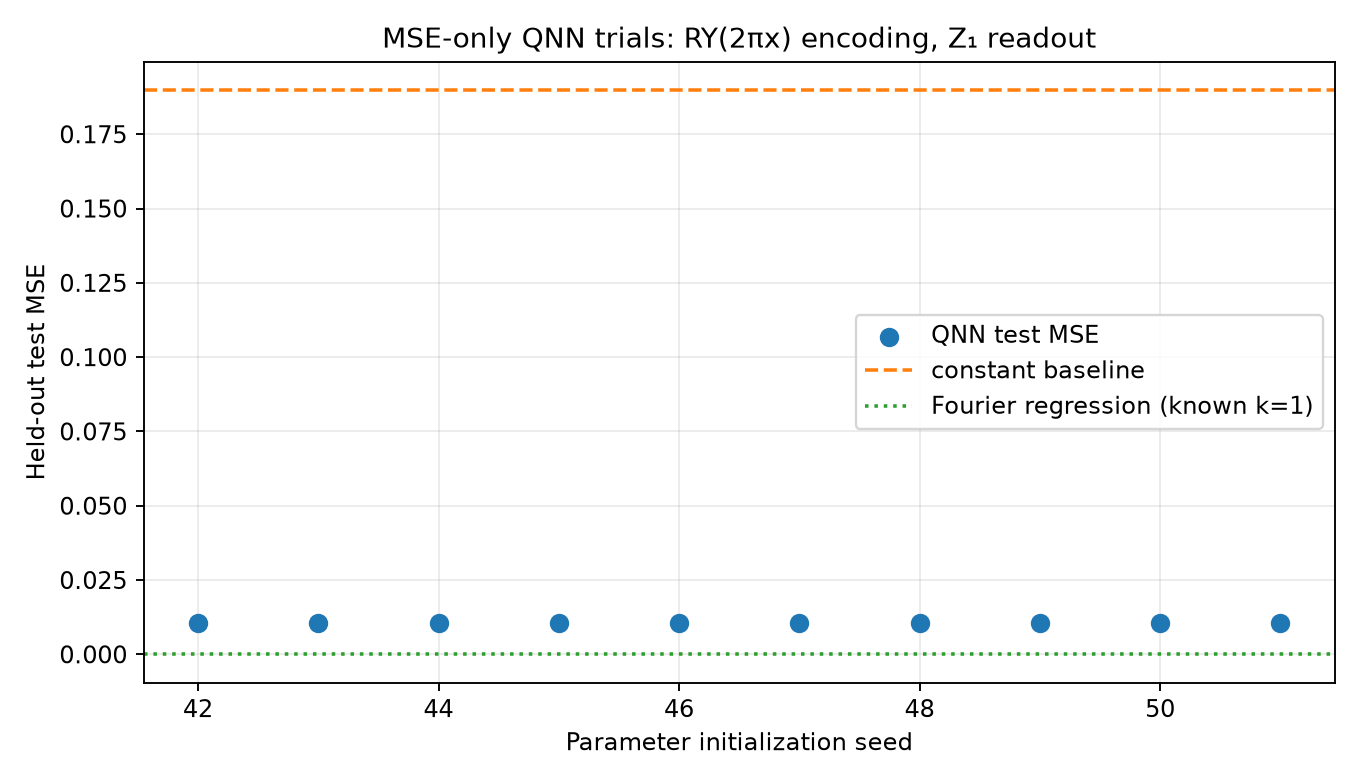
\includegraphics[width=0.84\linewidth]{results/periodic-function-mse-z1-readout/trial_test_mse.png}
  }{\fbox{Run the experiment to generate the grouped trial plot.}}
  \caption{Held-out MSE for the ten random initializations in the nonzero-offset experiment, with constant and known-frequency Fourier baselines.}
\end{figure}

\section{Run records and reproducibility}

Each invocation creates a unique, portable run bundle. Keep the resolved configuration, source revision/fingerprint, dependency versions, seeds, dataset and split metadata, parameter initialization, per-step metrics, parameter trajectory, final parameters, held-out predictions, summary metrics, plots, and HTML report. Store scalar run parameters and metric histories in MLflow when tracking is configured; keep the local structured bundle as the durable reanalysis record. MLflow is an index and tracking interface, not the only copy of the data.

Recommended artifacts include a JSON manifest and summary, resolved TOML/JSON configuration, \texttt{dataset.npz}, \texttt{metrics.jsonl}, \texttt{evaluation_outputs.npz}, parameter JSON/NPZ files, SVG or PNG plots, and \texttt{report.html}. Log the target coefficients in evaluation metadata, while keeping them out of the optimizer inputs. Store per-example predictions and targets so visualizations and metrics can be recomputed without rerunning training. For SLURM runs, record job/array IDs and requested resources; use the same runner and config semantics as local runs. Local two-qubit ideal simulation is suitable for development and small seed runs, while cluster resources are useful for larger sweeps, finite-shot sampling, noise studies, and longer experiments.

\section{Interpretation and lab decision}

Interpret each run on two axes. The circuit-recovery axis asks whether the learned input-independent unitary matches the canonical QFT, primarily using phase-insensitive process fidelity (and, secondarily, global-phase-aligned matrix error). The task axis asks whether the trained model predicts held-out targets and recovers the target Fourier support within predeclared tolerances. A run can succeed on either axis, both, or neither. Function MSE training does not contain enough information in general to identify a unique full unitary, so low MSE with low QFT fidelity is a meaningful task success but not algorithm recovery.

The current evidence shows examples of task success without full QFT recovery: zero-offset, single-frequency fits reached near-numerical-zero MSE while process fidelity remained low. Re-uploading also improved multi-frequency task fits, but changed the data-dependent circuit and increased trainable depth and parameter count together. This evidence motivates a lab decision, not a conclusion that re-uploading or any alternate encoding is the preferred ansatz. Candidate next studies include (i) fixed encoding variants with the original trainable block and parameter count held constant, (ii) re-uploading with a matched-depth single-upload control, and (iii) direct QFT recovery from randomized initialization. The group should choose the next branch and its success tolerances before launching another sweep.

\section{Interpretation and limitations}

Each outcome answers a bounded question for a specified circuit, target, data distribution, simulator, and optimizer budget. Results do not establish arbitrary-function learning, generalization outside the tested distribution, robustness to noise, or quantum advantage. A period-one angle encoding is appropriate to the chosen periodic domain and is not a universal encoding for nonperiodic data. Changing the fixed encoding can preserve the trainable gate layout while changing the model's function class; adding data re-uploading changes the input-dependent circuit structure, and adding blocks also changes trainable capacity. These distinctions must remain explicit in analysis.

\section{Implementation status}

The repository contains executable QFT-recovery and MSE function-learning experiments, including the completed single-frequency, multi-dataset, component-count, and data re-upload studies described above. This methodology records their interpretation and the controls required for future comparisons. Update this status as new protocols are selected and completed.

\begin{thebibliography}{9}
\bibitem{schuld2021}
M. Schuld, R. Sweke, and J. J. Meyer,
\newblock ``The effect of data encoding on the expressive power of variational quantum-machine-learning models,''
\newblock \emph{Physical Review A}, vol. 103, 032430, 2021.
\newblock \href{https://doi.org/10.1103/PhysRevA.103.032430}{doi:10.1103/PhysRevA.103.032430}.
\bibitem{perez2020}
A. P\'erez-Salinas, A. Cervera-Lierta, E. Gil-Fuster, and J. I. Latorre,
\newblock ``Data re-uploading for a universal quantum classifier,''
\newblock \emph{Quantum}, vol. 4, p. 226, 2020.
\newblock \href{https://doi.org/10.22331/q-2020-02-06-226}{doi:10.22331/q-2020-02-06-226}.
\end{thebibliography}

\end{document}
